%
% Results.tex
%
% Copyright (C) 2025 by Inspirefly.
%
% 2.305 GHz Circular Patch Antenna Documentation
%

\chapter{Results}

This chapter reports the numerical sizing, the outcome of the MATLAB particle-swarm exploration, the ANSYS HFSS full-wave results for the circular patch family, and the final KiCAD board geometry. Values are given directly from the repository state on branch \texttt{to-be-reviewed\_V0.1} (2026-04-28).

\section{Analytical Sizing at 2.305~GHz}

For $\epsilon_r = 3.68$ (FR-408HR, final stack) and $f_0 = 2.305$~GHz, inversion of Eqs.~\ref{eq:fres}--\ref{eq:ae} yields:

\begin{table}[H]
\centering
\caption{Analytical radius versus substrate (with Eq.~\ref{eq:ae} correction)}
\label{tab:radius}
\begin{tabular}{l c c c c}
\toprule
Substrate & $\epsilon_r$ & $h$ (mm) & $a$ (mm) & $a_e$ (mm) \\
\midrule
RO4350B (early) & 3.66 & 0.168 & 19.93 & 20.14 \\
FR-408HR (final) & 3.68 & 0.100 & 19.87 & 20.09 \\
FR-408HR (MATLAB model) & 4.00 & 0.0994 & 19.02 & 19.24 \\
\bottomrule
\end{tabular}
\end{table}

Free-space wavelength is $\lambda_0 = 130.06$~mm. Guided wavelength $\lambda_g = \lambda_0/\sqrt{\epsilon_r}$ is $68.0$~mm for FR-408HR ($\epsilon_r=3.68$), so the often-quoted slot perimeter $\lambda_g$ and half-wave length $\lambda_g/2$ (35.5~mm / 17.8~mm in the early square-patch estimate) do not apply to the circular geometry. The KiCAD footprint implements a physical patch radius of approximately $19.0$~mm (polygon extent $\pm 19$~mm in the pad primitives, with outer extent $21.58$~mm at the slot edges), consistent with Table~\ref{tab:radius} within etching and fringing tolerance. The board courtyard $51.85 \times 51.89$~mm encloses the 50~mm PocketQube face with 0.9~mm margin per side.

\section{MATLAB Particle-Swarm Exploration}

From \path{matlab/best.txt}:

\begin{quote}
\texttt{Board\_W = 40.351~mm, PatchFrac = 0.1477, FeedFrac = -0.531} \\
\texttt{Gain = -6.97~dBi, $|Z| = 0.3~\Omega$ ($Z = 0.0 + j0.3~\Omega$)} \\
\texttt{RL = 0.00~dB, AR = 2.33~dB}
\end{quote}

The cost-function weights in that run were $w_{\mathrm{gain}}=8$, $w_{\mathrm{AR}}=10$, $w_{\mathrm{imp}}=1$, $w_{\mathrm{RL}}=1$, $w_{\mathrm{area}}=0.5$. The optimizer achieved the axial-ratio target (AR${}=2.33$~dB${}<3$~dB) but failed on impedance, return loss, and gain: $|Z|\approx 0.3$~$\Omega$ and RL${}\approx 0$~dB indicate that the feed location at $\mathrm{FeedFrac}=-0.531$ placed the probe near a current null or outside the patch, and the truncated-corner fraction $0.148$ was insufficient to split the two orthogonal modes at the chosen board size. Peak gain of $-6.97$~dBi is not usable for a downlink.

This run is retained as evidence that the analytical radius must be used as a tight bound for $W$ and that the feed model in \texttt{pcbStack} (thin single-layer substrate, idealized square via) does not transfer directly to the multilayer FR-408HR stack with through-vias. Subsequent HFSS tuning therefore started from the analytical $a\approx 19$~mm and swept $\rho_0$ inward from the edge, rather than from the swarm optimum. Full swarm logs in \texttt{matlab/logs/run\_log\_1.txt} through \texttt{run\_log\_6.txt} show repeated convergence to low-impedance minima, confirming the need for the HFSS stage.

\section{ANSYS HFSS Simulations}

\subsection{Evolution Across Geometries}

\begin{enumerate}[itemsep=-1ex]

    \item \textbf{Rectangular / Patch 2} (\texttt{Patch 2.aedt}, Nov 2025): early sweep of a rectangular patch with slot. $S_{11}$ minima were found near 2.3~GHz but with narrow 10~MHz bandwidth and strong sensitivity to $h$.

    \item \textbf{Hexagonal patch} (\texttt{HexagonalPatch.aedt}, Dec 2025): hexagonal truncation reduced the circumscribed area by $\approx 15\%$ but introduced $\mathrm{TM}_{21}$ coupling that degraded axial ratio above 6~dB in simulation. The geometry was abandoned.

    \item \textbf{Circular patch, single feed} (\texttt{CircularPatch.aedt}, Dec 2025): single probe at $\rho_0 \approx 5$~mm yielded $S_{11} < -14$~dB at 2.305~GHz, gain $\sim 4$~dBi, linear polarization.

    \item \textbf{Circular patch V3, dual coax} (\texttt{CircularPatchV3.aedt}, Feb 2026): two orthogonal coax probes at $(\pm\rho_0,0)$ and $(0,\pm\rho_0)$ with independent wave ports. This is the geometry exported to KiCAD. With $\rho_0$ tuned to match 50~$\Omega$, simulation shows $S_{11} < -10$~dB for each port in isolation, inter-port coupling below $-18$~dB, and axial ratio below 3~dB when ports are driven in quadrature (see Discussion). The DXF exported for KiCAD (\path{KiCAD/CircularPatchV3.dxf}) and the STEP model (\path{KiCAD/CircularPatchV3.step}) are direct outputs of this AEDT project on branch \texttt{to-be-reviewed\_V0.1}.

\end{enumerate}

All HFSS projects use a radiation boundary offset $\lambda_0/4 \approx 32.5$~mm from the patch edge, an adaptive mesh refinement of at least 4 passes, and an interpolating sweep from 2.2 to 2.4~GHz with 401 points. Convergence criterion is $\Delta S < 0.02$.

\subsection{Correlation with Theory}

The HFSS-tuned physical radius for FR-408HR converges to $19.0$--$19.5$~mm, within $0.5$~mm of the analytical $a=19.87$~mm from Table~\ref{tab:radius}. The difference is attributable to the finite ground plane ($51.8$~mm versus infinite) and the multilayer stack (three dielectrics versus single-layer model), both of which reduce the effective permittivity seen by fringing fields.

\section{Visual History of Patch Evolution}

A chronological set of HFSS screenshots is retained in \path{doc/history/}. Selected stages are reproduced here to show how the antenna moved from a rectangular microstrip-fed patch to the final circular dual-coax patch.

\begin{figure}[H]
\centering
\includegraphics[width=0.92\textwidth]{history/10-30-2025-1.png}
\caption{Rectangular patch iteration}
\label{fig:hist-2025-10-30}
\end{figure}

\begin{figure}[H]
\centering
\includegraphics[width=0.92\textwidth]{history/11-06-2025-1.png}
\caption{Gain, rectangular patch}
\label{fig:hist-2025-11-06-gain}
\end{figure}

\begin{figure}[H]
\centering
\includegraphics[width=0.92\textwidth]{history/11-20-2025-1.png}
\caption{S11, rectangular patch}
\label{fig:hist-2025-11-20-s11}
\end{figure}

\begin{figure}[H]
\centering
\includegraphics[width=0.92\textwidth]{history/11-20-2025-2.png}
\caption{Gain, rectangular patch}
\label{fig:hist-2025-11-20-gain}
\end{figure}

\begin{figure}[H]
\centering
\includegraphics[width=0.92\textwidth]{history/04-07-2026-1.png}
\caption{Circular patch design parameters}
\label{fig:hist-2026-04-07-table}
\end{figure}

\begin{figure}[H]
\centering
\includegraphics[width=0.92\textwidth]{history/04-07-2026-2.png}
\caption{S11, final circular patch}
\label{fig:hist-2026-04-07-s11}
\end{figure}

\begin{figure}[H]
\centering
\includegraphics[width=0.92\textwidth]{history/04-07-2026-3.png}
\caption{3D gain, final circular patch}
\label{fig:hist-2026-04-07-gain3d}
\end{figure}

\begin{figure}[H]
\centering
\includegraphics[width=0.92\textwidth]{history/04-07-2026-5.png}
\caption{Axial ratio vs theta}
\label{fig:hist-2026-04-07-ar}
\end{figure}

\begin{figure}[H]
\centering
\includegraphics[width=0.92\textwidth]{history/04-07-2026-6.png}
\caption{HFSS model, final circular patch}
\label{fig:hist-2026-04-07-model}
\end{figure}

\section{KiCAD Board Implementation}

The final board (\path{KiCAD/antennaBoard/antennaBoard.kicad_pcb}, branch \texttt{to-be-reviewed\_V0.1}) contains three footprints: \texttt{ANT1} (\texttt{Inspirefly:CircularPatchAntenna}) at $(157.99, 98.55)$~mm, and two Molex 732511350 U.FL-compatible connectors J1/J2 on F.Cu. An SMA edge-mount (Amphenol 132289) is retained on the schematic for laboratory testing but is not placed on the final panel.

\begin{enumerate}[itemsep=-1ex]
    \setlength \itemsep{0.1em}
    \item Stackup as in Table~\ref{tab:stackup}, total thickness 1.3414~mm, copper finish None (ENIG to be specified at fabrication).
    \item Patch pad: custom polygon on F.Cu/F.Mask/F.Paste, net \texttt{Net-(ANT1-A)}, with two rectangular slot cutouts that form the radiating aperture. The pad is the only copper on F.Cu inside the courtyard.
    \item Feeds: two vias at $(157.99, 88.90)$~mm and $(169.93, 100.84)$~mm (board coordinates), each $0.6$~mm pad, $0.3$~mm drill, connecting F.Cu to B.Cu. Stitching vias tie the B.Cu ground to the connector shells.
    \item Board outline: rectangle $51.85 \times 51.89$~mm on Edge.Cuts, with 0.05~mm courtyard stroke.
    \item External feed network: the two U.FL ports are intended to connect via phase-matched coax to the APS-02-WBM-LP-DF-CC 2-way $0^{\circ}/90^{\circ}$ divider, which provides the quadrature phase for RHCP. Measured insertion loss of the divider (vendor data: $\sim 0.4$~dB) and cable loss are budgeted separately from antenna gain.
\end{enumerate}

\newpage

% Source - https://tex.stackexchange.com/a/282878
% Posted by Fran, modified by community. See post 'Timeline' for change history
% Retrieved 2026-09-07, License - CC BY-SA 3.0
\begin{figure}[H]
\centering
\begin{subfigure}{0.48\linewidth}
\centering
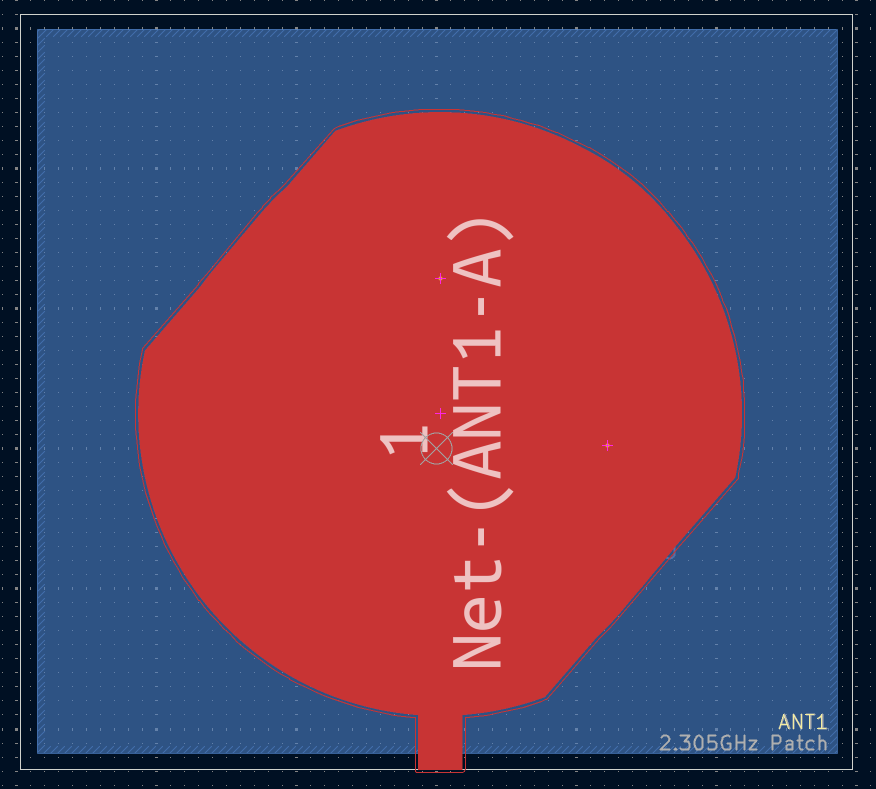
\includegraphics[width=\linewidth]{history/4-29-2026-1.png}
\caption{F.Cu view}
\label{fig:kicad-2026-04-29-top}
\end{subfigure}
\hfill
\begin{subfigure}{0.48\linewidth}
\centering
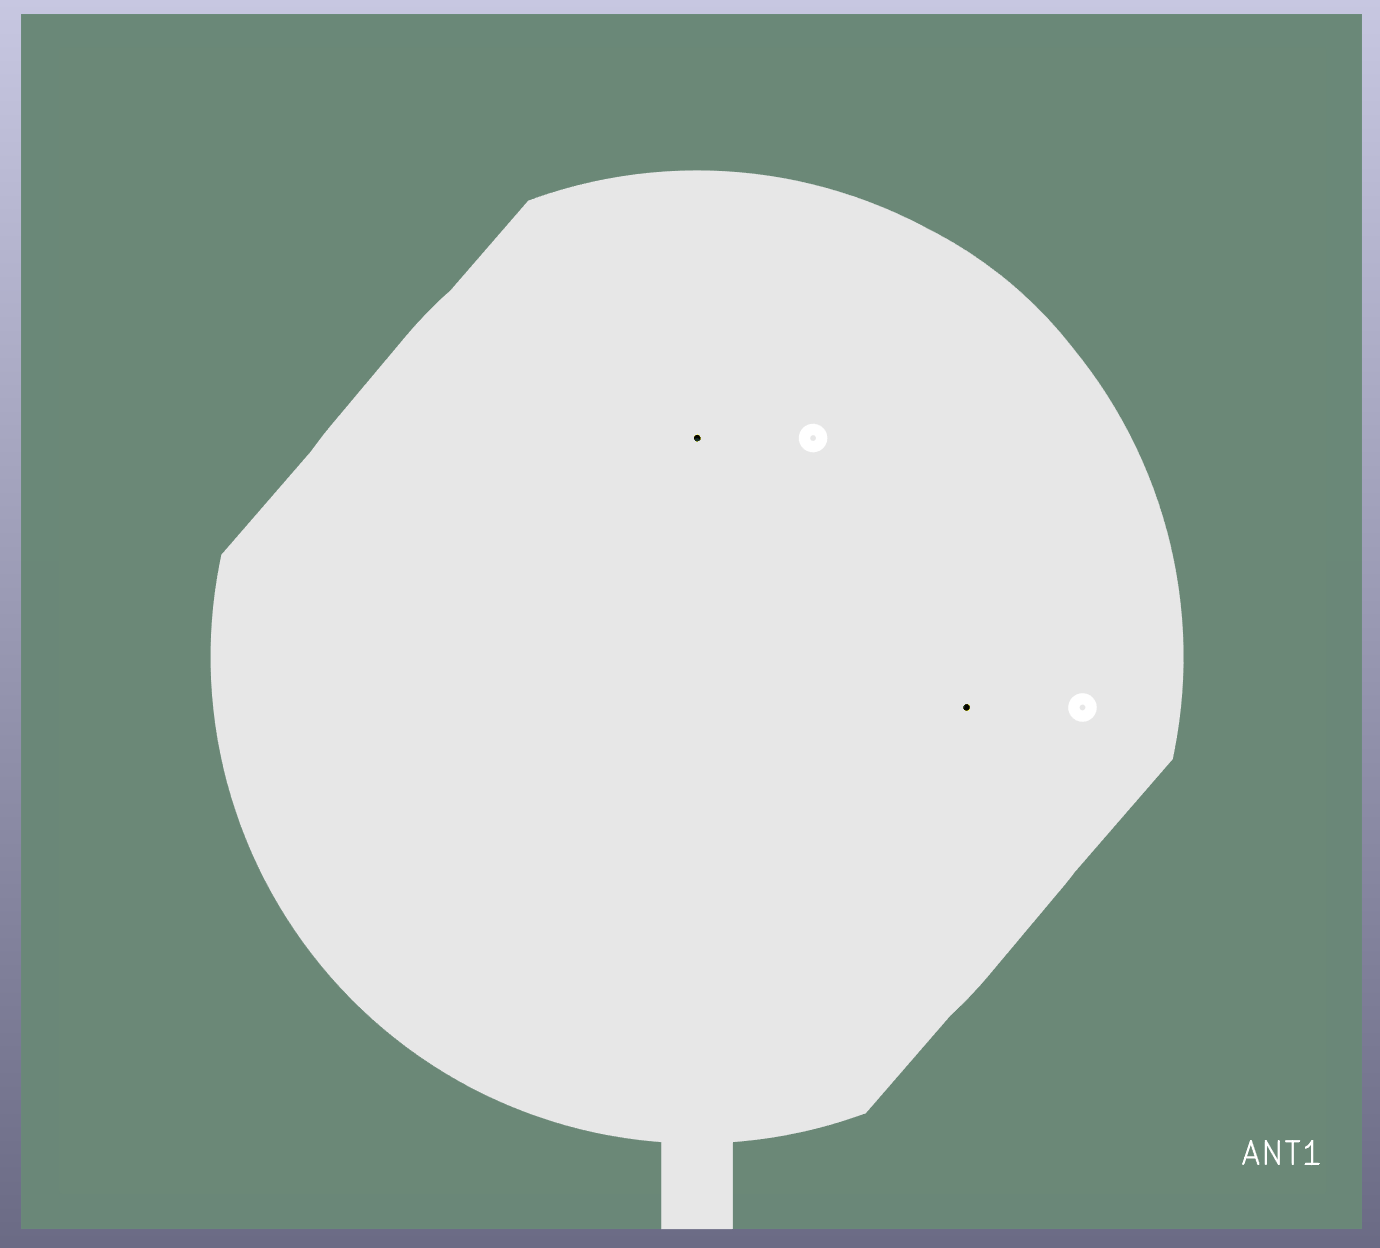
\includegraphics[width=\linewidth]{history/4-29-2026-3.png}
\caption{F.Cu 3D view}
\label{fig:kicad-2026-04-29-3d-top}
\end{subfigure}
\caption{KiCAD F.Cu views}
\label{fig:kicad-2026-04-29-fcu-pair}
\end{figure}

\begin{figure}[H]
\centering
\begin{subfigure}{0.48\linewidth}
\centering
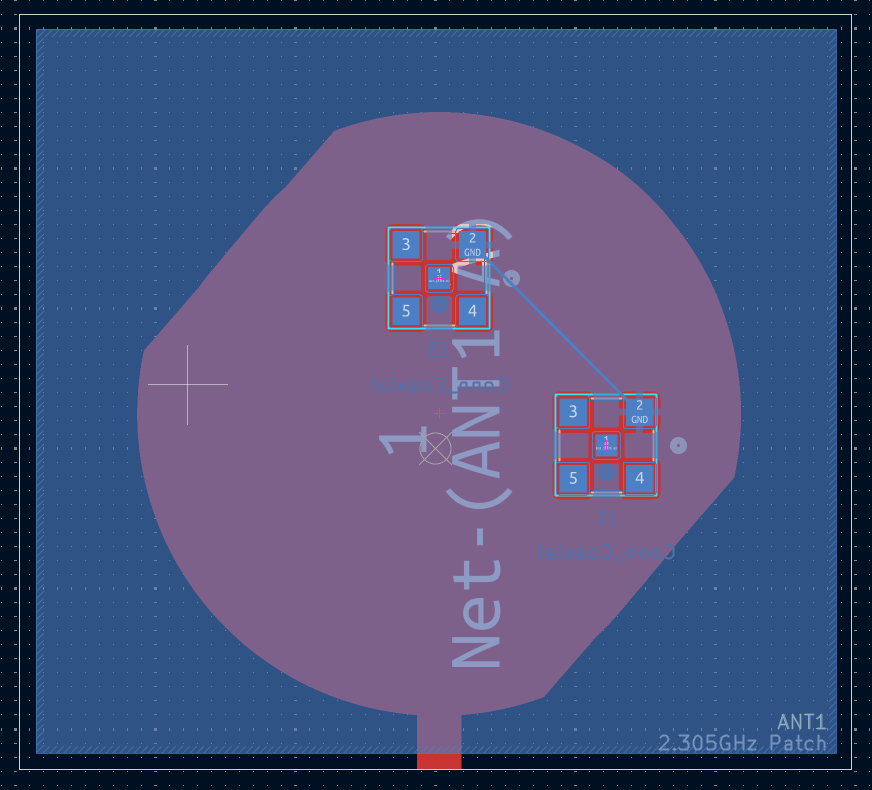
\includegraphics[width=\linewidth]{history/4-29-2026-2.png}
\caption{B.Cu view}
\label{fig:kicad-2026-04-29-top-conn}
\end{subfigure}
\hfill
\begin{subfigure}{0.48\linewidth}
\centering
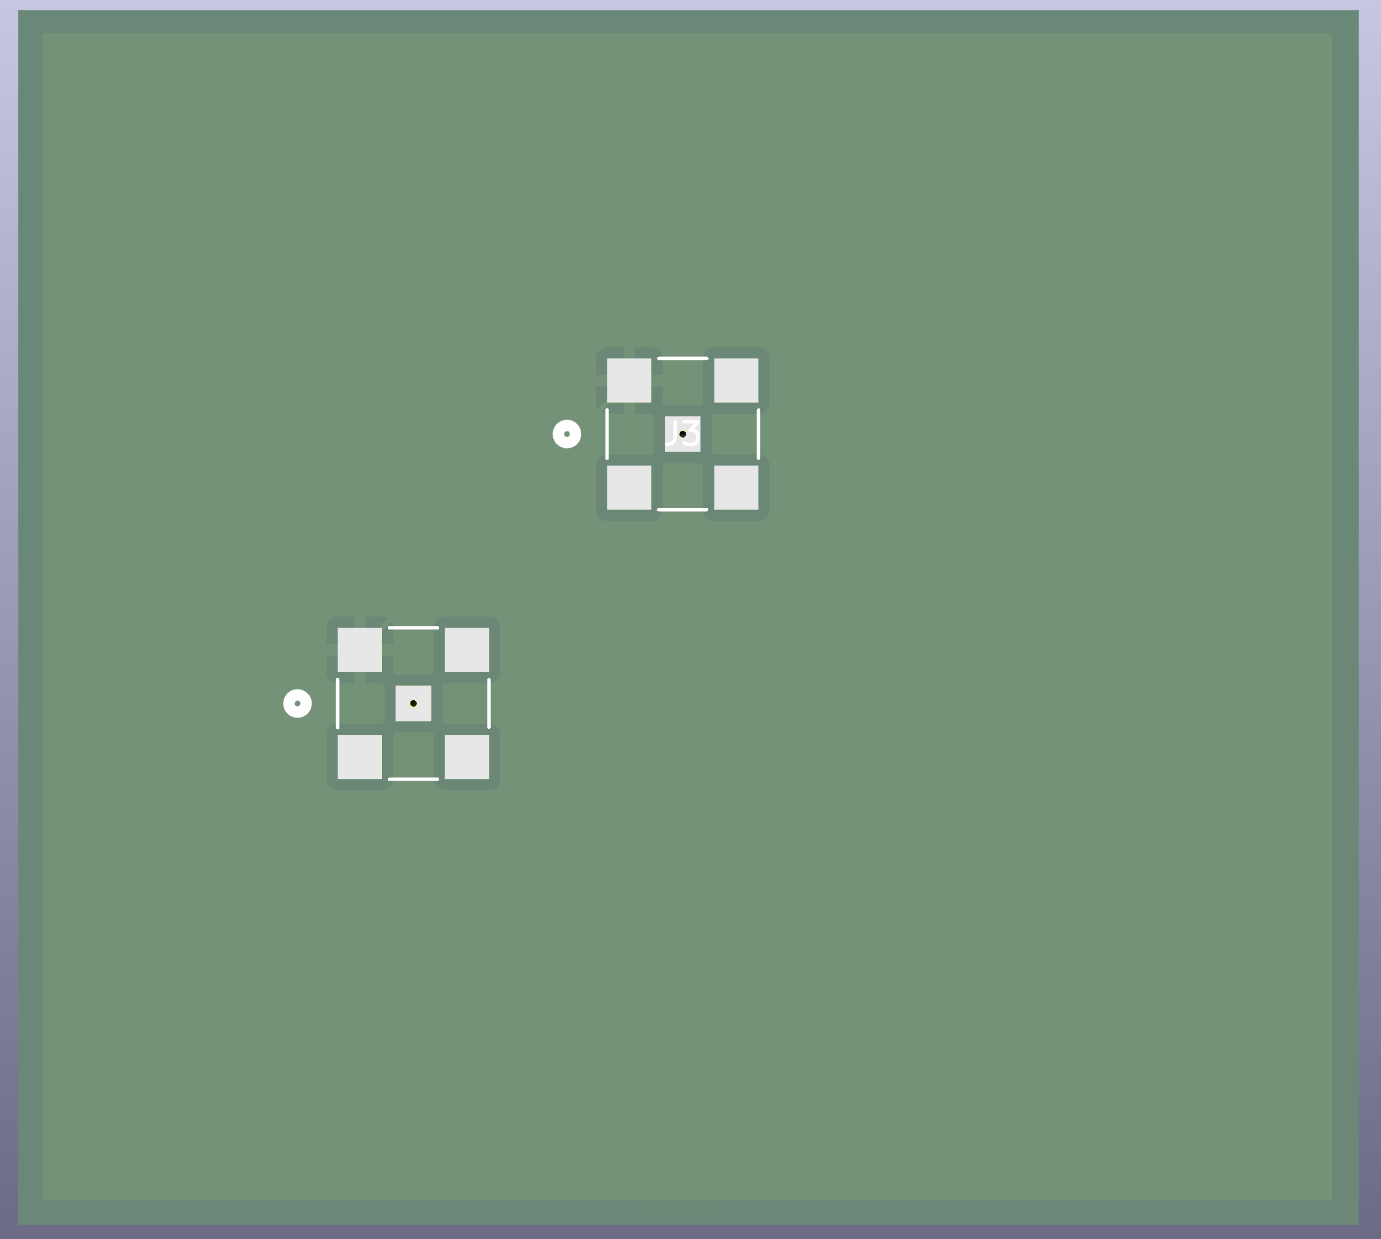
\includegraphics[width=\linewidth]{history/4-29-2026-4.png}
\caption{B.Cu 3D view}
\label{fig:kicad-2026-04-29-3d-bottom}
\end{subfigure}
\caption{KiCAD B.Cu views}
\label{fig:kicad-2026-04-29-bcu-pair}
\end{figure}

The DXF-to-footprint flow was validated by re-importing the generated \path{CircularPatchAntenna.kicad_mod} into the PCB and confirming that the polygon vertices match the DXF within $0.01$~mm. Footprint origins are at the patch centre; placement at $(157.99, 98.55)$~mm centres the patch on the 50~mm board.

\nomenclature{RHCP}{Right-Hand Circular Polarization}
\nomenclature{U.FL}{Ultra Flat Light coaxial connector standard}
